\documentclass{article}
\usepackage{pgfplots}
\usepackage[T1]{fontenc}
\usepackage[utf8]{inputenc}
\usepackage{stanli} % TikZ Library for Structural Analysis by Jurgen Hackl
\usetikzlibrary{calc,intersections,patterns}
\usepackage{graphics,mathtools}
\usepackage{tikz}
\usepackage{palatino}

\usetikzlibrary{external}
\tikzexternalize[prefix=tikzout/]


\begin{document}
Our figures
% Rest of preamble
% Begin document, write stuff

%% Set a filename for the next tikzpicture.
%\tikzsetnextfilename{fr181451}
%\begin{tikzpicture}
%\begin{axis}[xlabel=\textbf{$\mathbf{v_{uv}/\phi v_c}$}, ylabel= \textbf{Design story drift ratio ($\mathbf{\Delta_x/h_{sx}}$)}, xmin = 0, ymin = 0, xmax = 0.75, ymax = 0.04, scaled ticks=false, xmajorgrids,ymajorgrids,xtick={0,0.1,0.2,0.3,0.4,.5,.6,.7},ytick={0,0.01,0.02,0.03,0.04},
%yticklabels={0,0.01,0.02,0.03,0.04}]
%    % \begin{axis}[%
%    %     width=4.521in,
%    %     height=2in,
%    %     scale only axis,
%    %     xmin=0,
%    %     xmax=73,xtick={6,12,18,24,30,36,42,48,54,60,66,72},
%    %     xticklabels={{3},{6},{9},{12},{15},{18},{21},{24},{27},{30},{33},{36}},
%    %     xlabel={Cycle},
%    %     ymin=-4.5,
%    %     ymax=5.5, xmajorgrids, ymajorgrids,
%    %     ylabel={Drift, \%},
%    %     every axis y label/.style=
%    %     {at={(ticklabel cs:0.5)},rotate=90,anchor=center},
%    %     ]
%        \addplot [color=orange, line width=1.0pt, forget plot]
%          table[row sep=crcr]{%
%        0	0.035\\
%        0.6 0.005\\
%        0.75 0.005\\
%        };
%        % \addlegendentry{Nonprestressed}
%\end{axis}
%\draw (0.2,0.01) node [anchor=south west] {\textbf{Shear reinforcement not required}};
%\draw (6,5) node [anchor=north east] {\textbf{Shear reinforcement required}};
%\end{tikzpicture}

%\tikzsetnextfilename{h74f1}
%\begin{tikzpicture}
%\draw (0,0) node [anchor=south west] {
\includegraphics[width=\columnwidth]{h74f1.pdf}};
%%\draw (6,5) node [anchor=north east] {\textbf{Shear reinforcement required}};
%%\draw[help lines,red] (0,0) grid (12,40);
%\draw (3,41.2) node [anchor=north,blue]{\Large\textbf{a) Steel plate}};
%\draw (9,41.2) node [anchor=north,blue]{\Large\textbf{b) Channel sections}};
%\draw (3,32.6) node [anchor=north,blue]{\Large\textbf{c) I-sections}};
%\draw (9,32.6) node [anchor=north,blue]{\Large\textbf{d) Collar}};
%\draw (3,24.8) node [anchor=north,blue]{\Large\textbf{e) Shearhead-SH cage}};
%\draw (9,24.8) node [anchor=north,blue]{\Large\textbf{f) Shearhead cage-SH}};
%\draw (3,16) node [anchor=north,blue]{\Large\textbf{g) Bent bars-B}};
%\draw (9,16) node [anchor=north,blue]{\Large\textbf{h) Bent bars-B}};
%\draw (3,7.6) node [anchor=north,blue]{\Large\textbf{i) Bent radial bars-BR}};
%\draw (9,7.6) node [anchor=north,blue]{\Large\textbf{j) Radial stirrups-RS}};
%\draw (3,0) node [anchor=north,blue]{\Large\textbf{k) Vertical stirrups-VS}};
%\draw (9,0) node [anchor=north,blue]{\Large\textbf{l) Inclined stirrups-IS}};
%\end{tikzpicture}
%\tikzsetnextfilename{h74f2}
%\begin{tikzpicture}
%\draw (0,0) node [anchor=south west] {
\includegraphics[width=\columnwidth,trim = 0 0 0 955px,clip]{h74f1.pdf}};
%\draw (0,-1) node [anchor=north west] {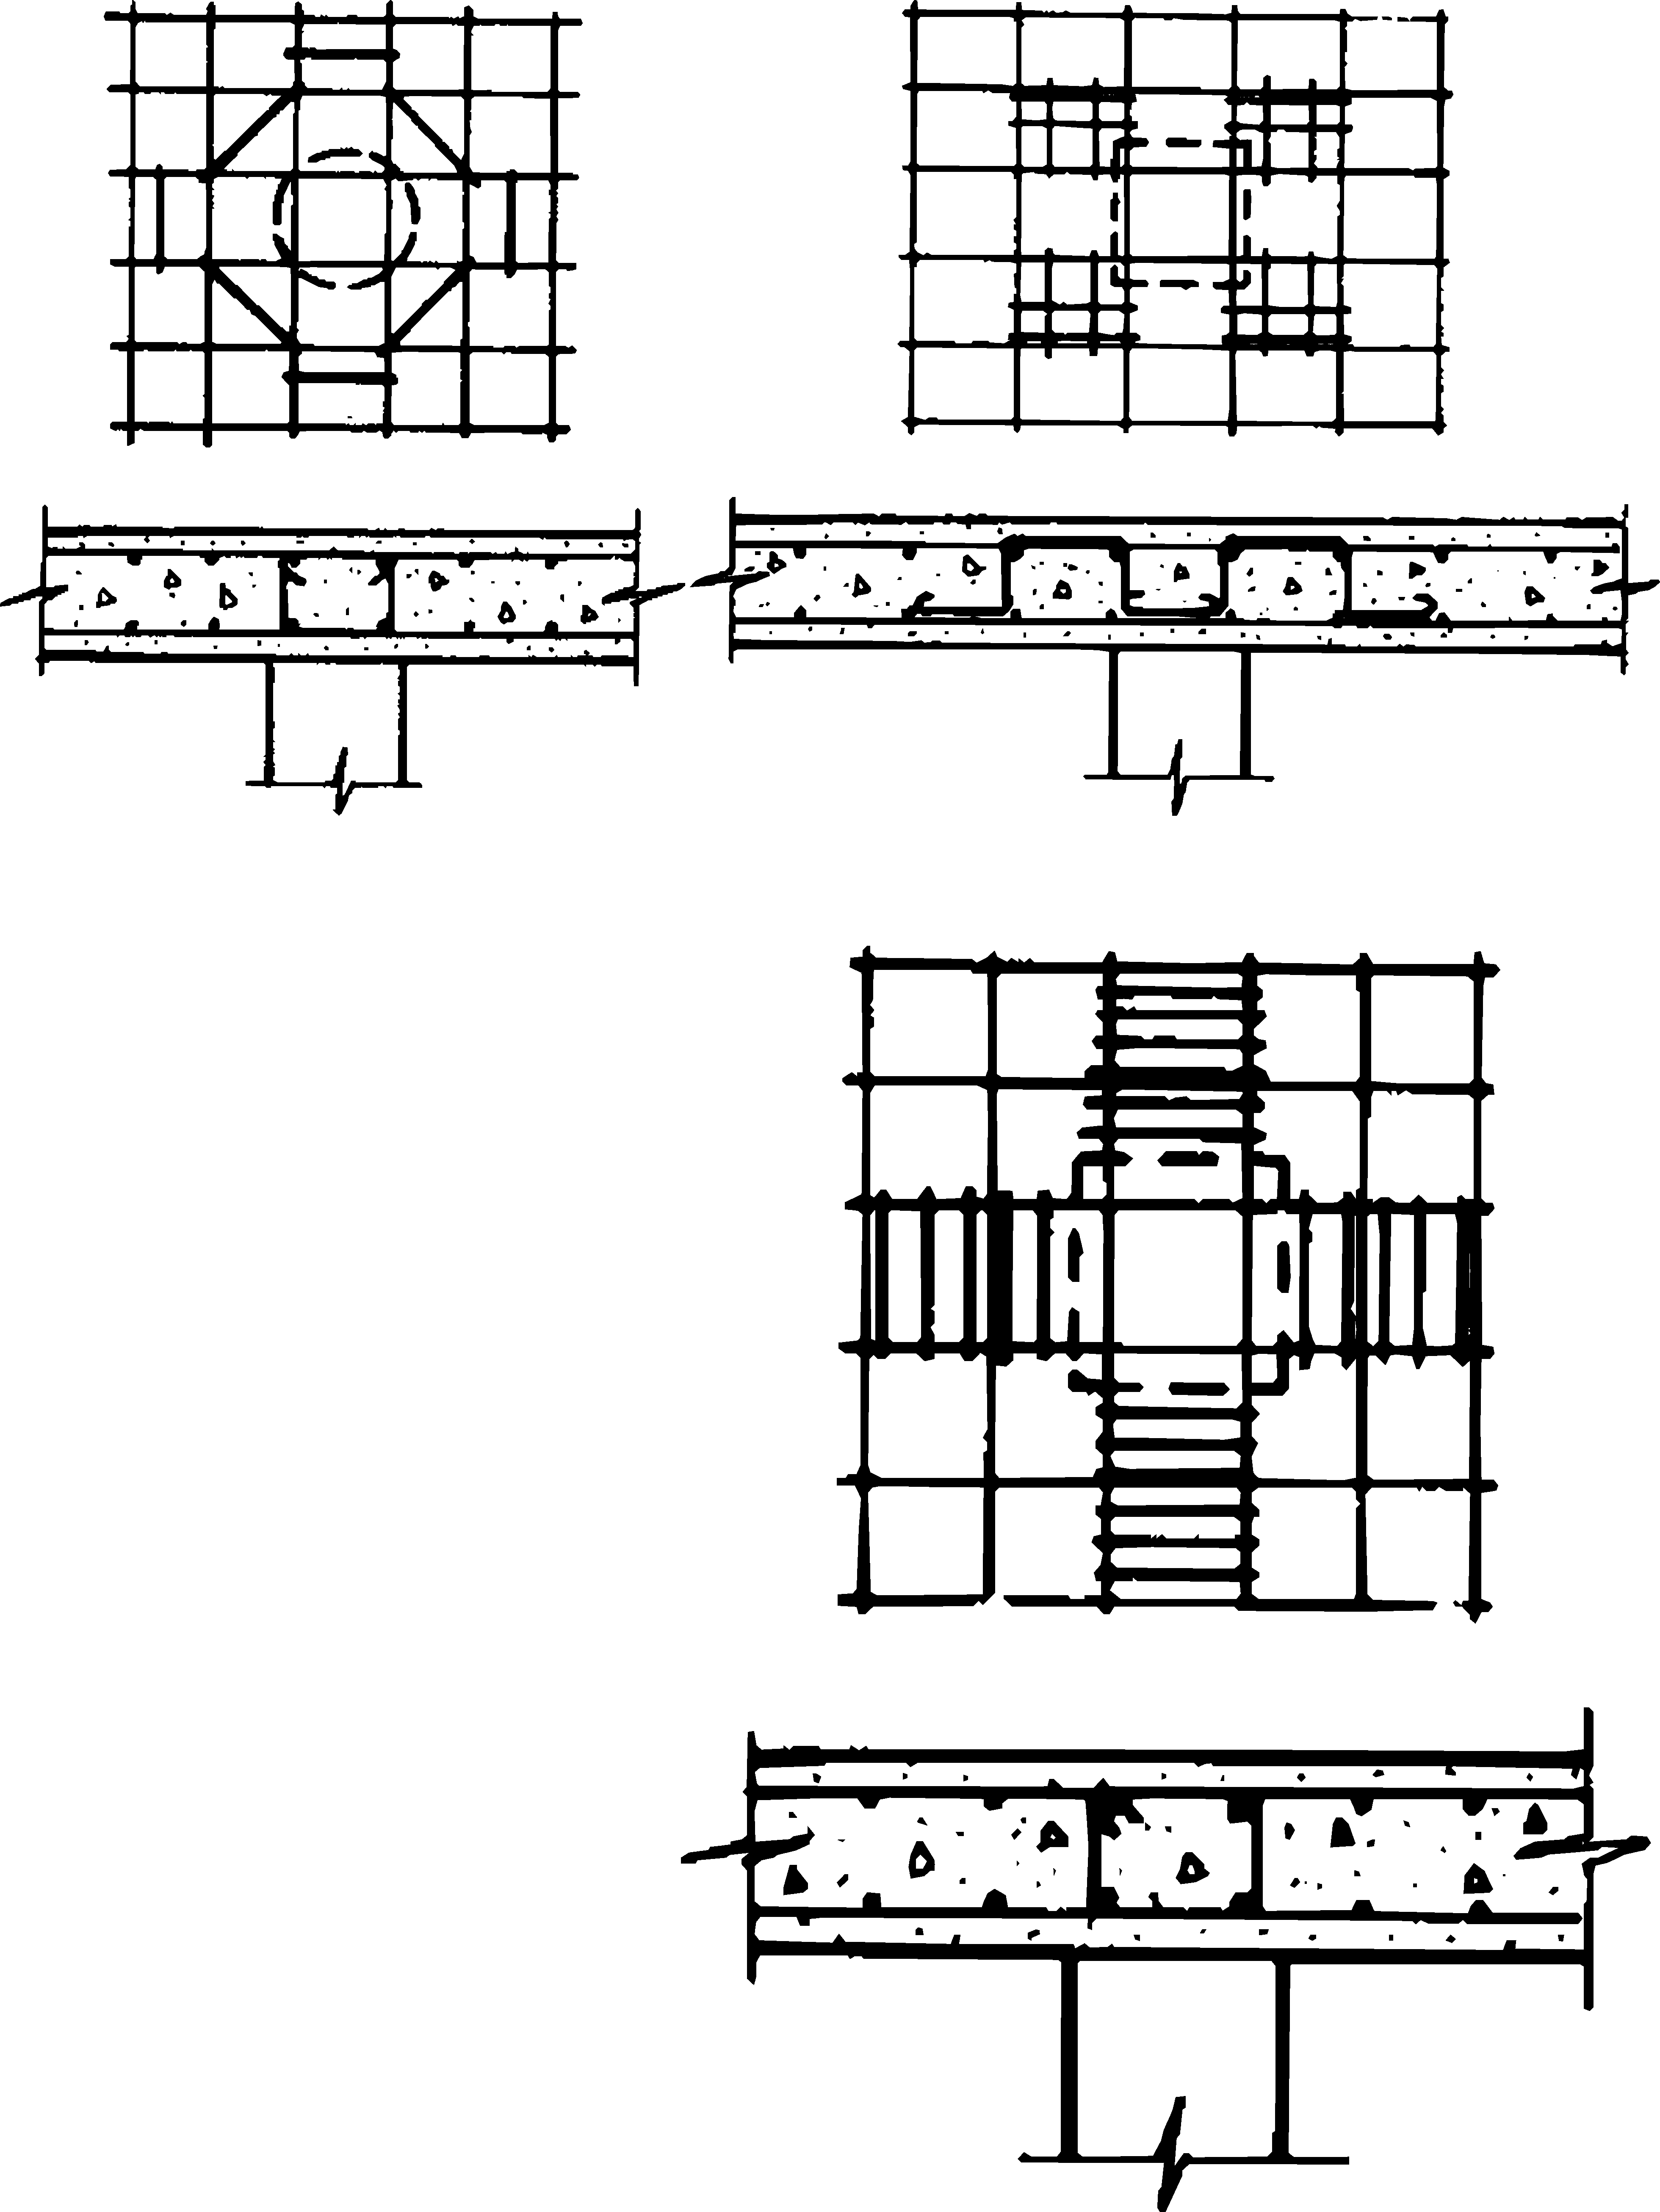
\includegraphics[width=\columnwidth]{h74f2.pdf}};
%
%%\draw (6,5) node [anchor=north east] {\textbf{Shear reinforcement required}};
%%\draw[help lines,red] (0,0) grid (12,40);
%\draw (3,7.6) node [anchor=north,blue]{\Large\textbf{i) Bent radial bars-BR}};
%\draw (9,7.6) node [anchor=north,blue]{\Large\textbf{j) Radial stirrups-RS}};
%\draw (3,0) node [anchor=north,blue]{\Large\textbf{k) Vertical stirrups-VS}};
%\draw (9,0) node [anchor=north,blue]{\Large\textbf{l) Inclined stirrups-IS}};
%\draw (3,-7) node [anchor=north,blue]{\Large\textbf{m) Closed stirrups-CS}};
%\draw (3,-7.8) node [anchor=north,blue]{\Large\textbf{ Radial-CSR}};
%\draw (3,-8.6) node [anchor=north,blue]{\Large\textbf{ Tangetial-CST}};
%\draw (9,-7) node [anchor=north,blue]{\Large\textbf{n) U-Shaped stirrups-US}};
%\draw (9,-17.2) node [anchor=north,blue]{\Large\textbf{o) Beam stirrups-BS}};
%\end{tikzpicture}

%\tikzsetnextfilename{fr2269814}
%\begin{tikzpicture}
%\draw (0,0) node [anchor=south west] {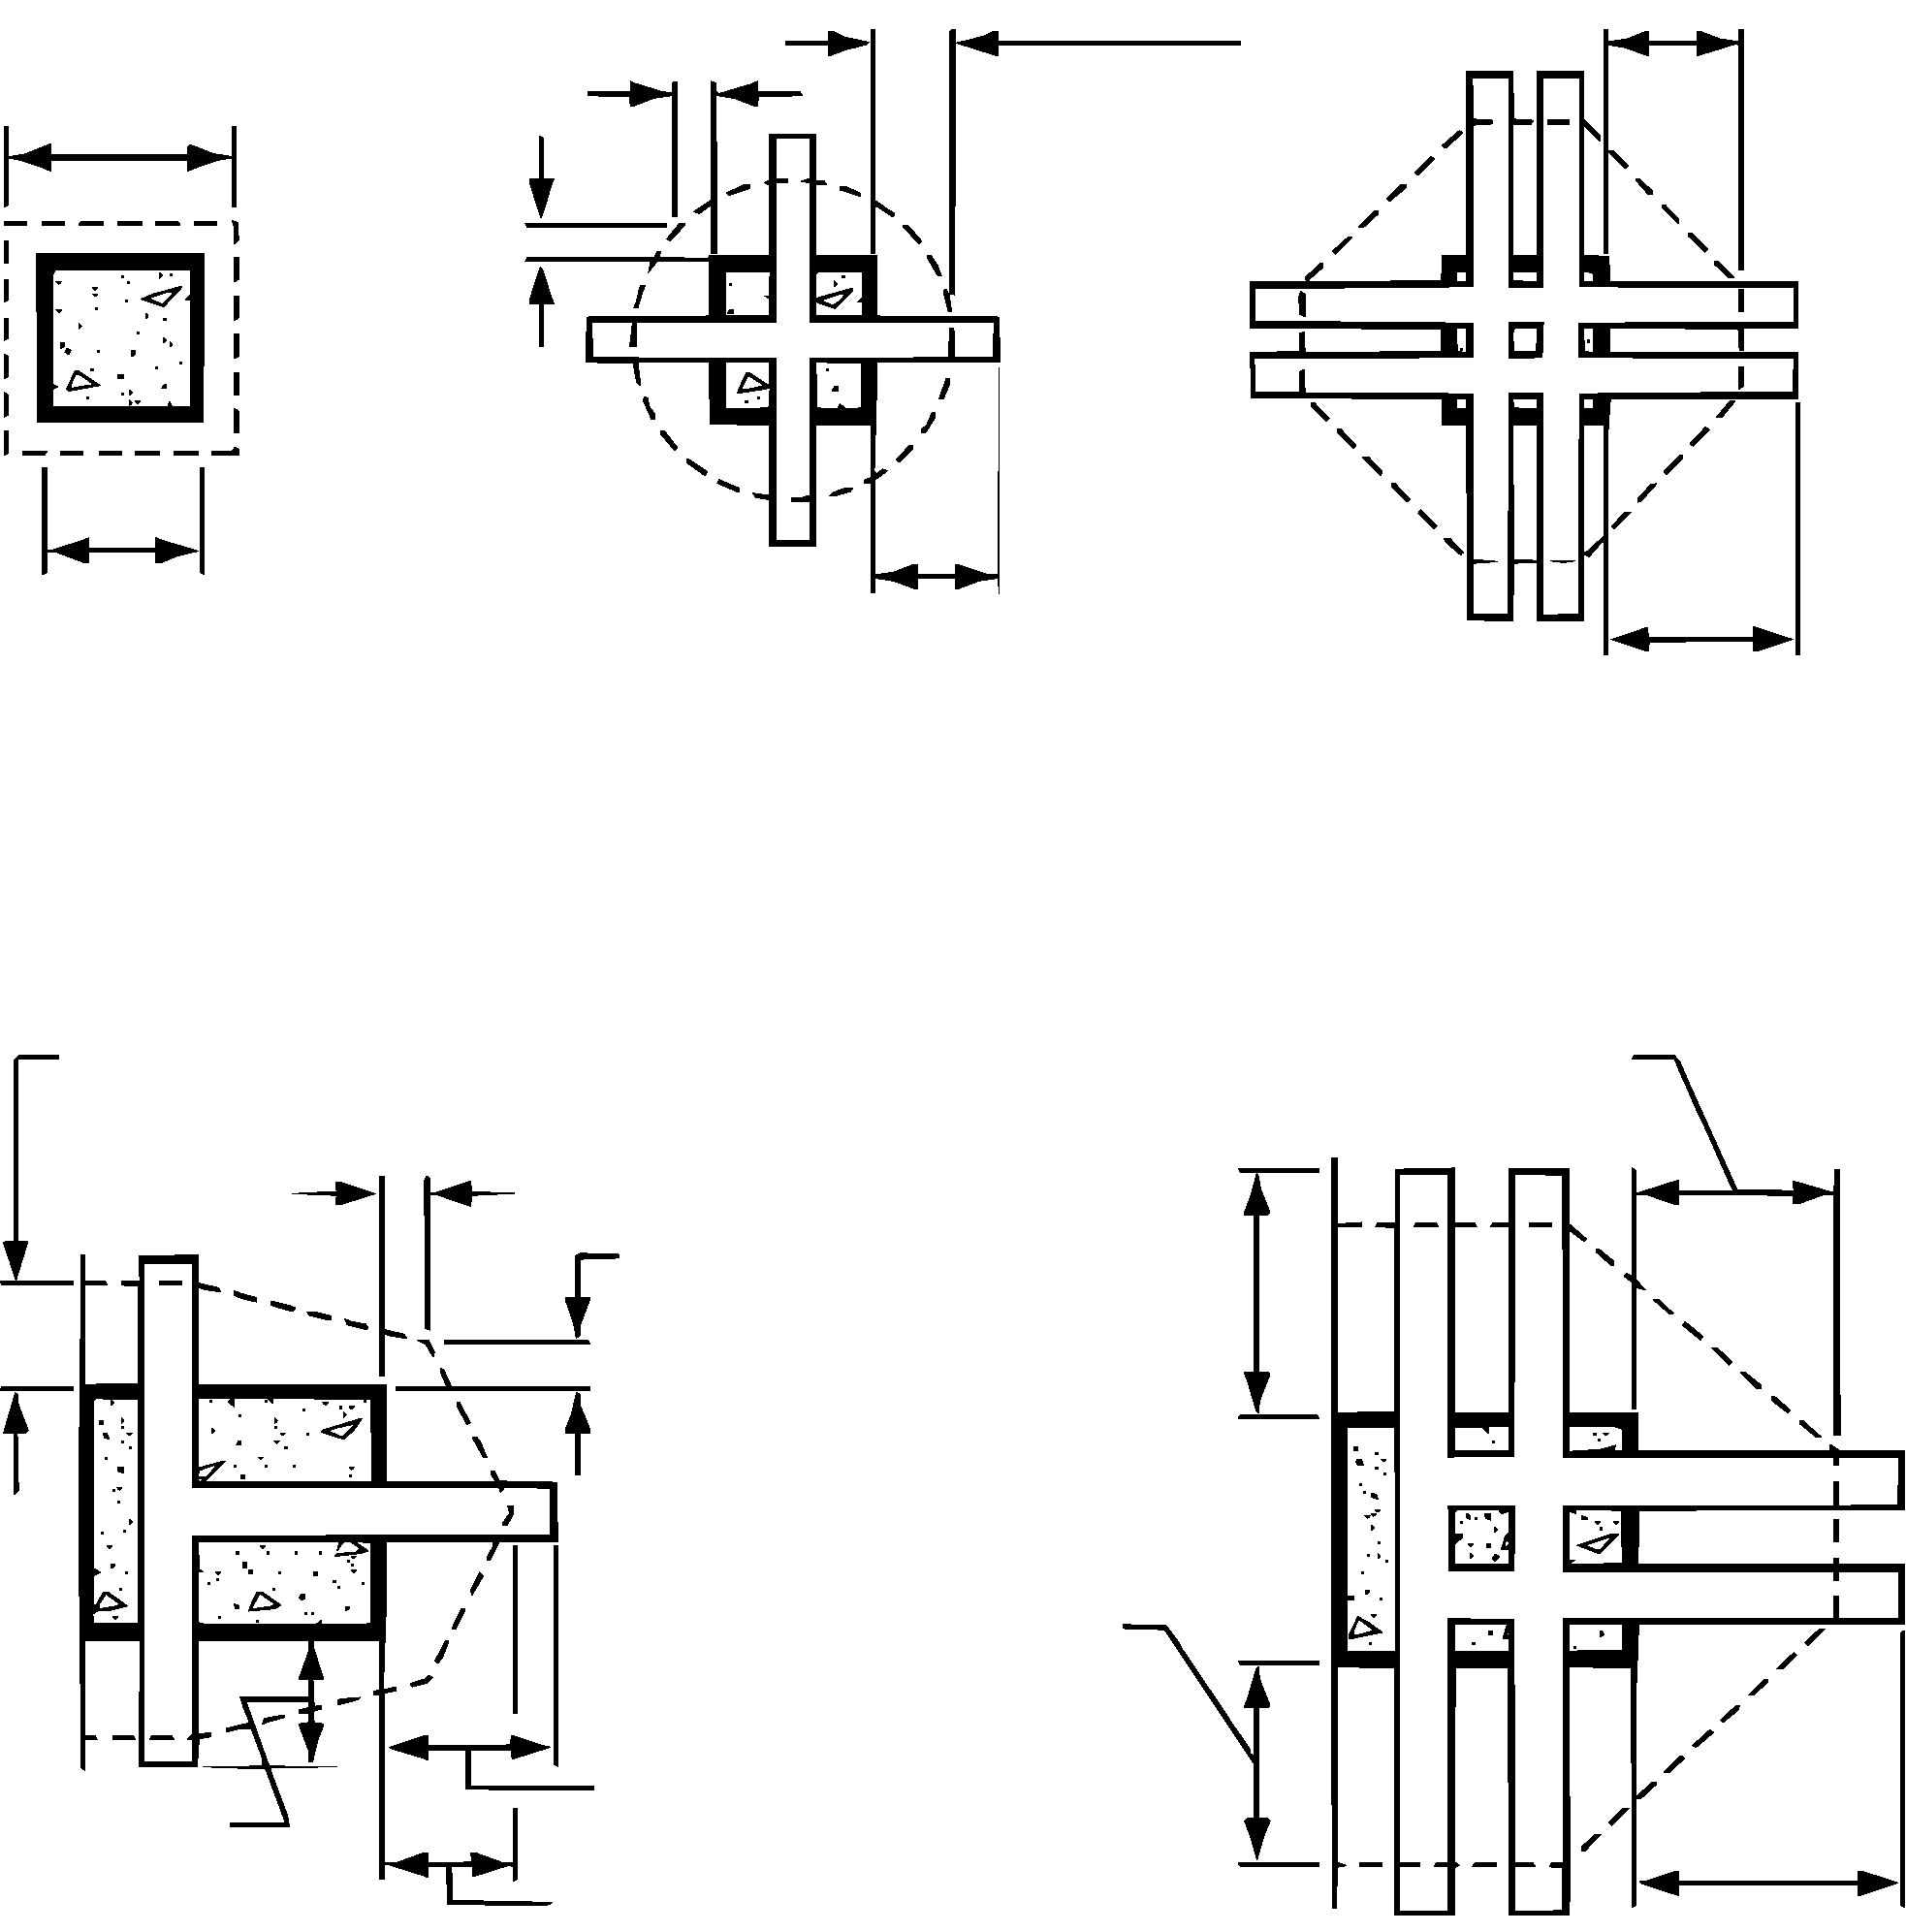
\includegraphics[width=\columnwidth]{fr2269814.pdf}};
%
%%\draw (6,5) node [anchor=north east] {\textbf{Shear reinforcement required}};
%%\draw[help lines,red] (0,0) grid (12,15);
%\draw (1.7,0.8) node [anchor=east]{\large$\mathbf{\ell_v-c_2}/2$};
%\draw (3.5,0.3) node [anchor=west]{\large$3/4\mathbf{(\ell_v-c_1}/2)$};
%\draw (3.9,1) node [anchor=west]{\large$\mathbf{\ell_v-c_1}/2$};
%\draw (2.8,1.25) node [anchor=south west]{\large$C'$};
%\draw (2.9,3.9) node [anchor=south west]{\large$B'$};
%\draw (7.3,2) node [anchor=east]{\large$3/4\mathbf{(\ell_v-c_2}/2)$};
%\draw (0.4,5.7) node [anchor=west]{\large$3/4\mathbf{(\ell_v-c_2}/2)$};
%\draw (2,5) node [anchor=north east]{\large$\mathbf{d}/2$};
%\draw (4,4.4) node [anchor=west]{\large$\mathbf{d}/2$};
%
%\draw (0,0) node [anchor=north west,blue]{\large\textbf{d) Small edge shearhead}};
%\draw (2.5,-0.5) node [anchor=north,blue]{\large($\mathbf{n}=3$)};
%
%\draw (10,-0.25) node [anchor=north,blue]{\large\textbf{e) Large edge}};
%\draw (10,-0.75) node [anchor=north,blue]{\large\textbf{shearhead}};
%\draw (10,-1.25) node [anchor=north,blue]{\large($\mathbf{n}=3$)};
%\draw (12.3,-0.1) node [anchor=east]{\large$\mathbf{\ell_v-c_1}/2$};
%\draw (10.65,0.1) node [anchor=south east]{\large$C'$};
%\draw (9.97,5.15) node [anchor=north west]{\large$B'$};
%\draw (8.1,4) node [anchor=south east]{\large$\mathbf{\ell_v-c_2}/2$};
%\draw (10.6,5.4) node [anchor=south east]{\large$3/4\mathbf{(\ell_v-c_1}/2)$};
%
%\draw (0.2,11.4) node [anchor=south west]{\large$\mathbf{c_1+d}$};
%\draw (1.25,8.85) node [anchor=south east]{\large$\mathbf{c_1}$};
%\draw (6,8.7) node [anchor=north]{\large$\mathbf{\ell_v-c_1}/2$};
%\draw (6.6,12.1) node [anchor=south]{\large$3/4\mathbf{(\ell_v-c_1}/2)$};
%\draw (3.5,10.8) node [anchor=east]{\large$\mathbf{d}/2$};
%\draw (4.5,11.7) node [anchor=south]{\large$\mathbf{d}/2$};
%
%\draw (0,8.7) node [anchor=north west,blue]{\large\textbf{a) No shearhead}};
%\draw (5.3,8.2) node [anchor=north,blue]{\large\textbf{b) Small interior}};
%\draw (5.3,7.7) node [anchor=north,blue]{\large\textbf{shearhead}};
%\draw (5.3,7.2) node [anchor=north,blue]{\large($\mathbf{n}=4$)};
%
%\draw (10.7,12.1) node [anchor=south]{\large$3/4\mathbf{(\ell_v-c_1}/2)$};
%\draw (10.9,8.4) node [anchor=north]{\large$\mathbf{\ell_v-c_1}/2$};
%\draw (10,7.9) node [anchor=north,blue]{\large\textbf{c) Large interior}};
%\draw (10,7.4) node [anchor=north,blue]{\large\textbf{shearhead}};
%\draw (10,6.9) node [anchor=north,blue]{\large($\mathbf{n}=4$)};
%
%\end{tikzpicture}
%\tikzsetnextfilename{ahf5}
%\begin{tikzpicture}
%\draw (0,0) node [anchor=south west] {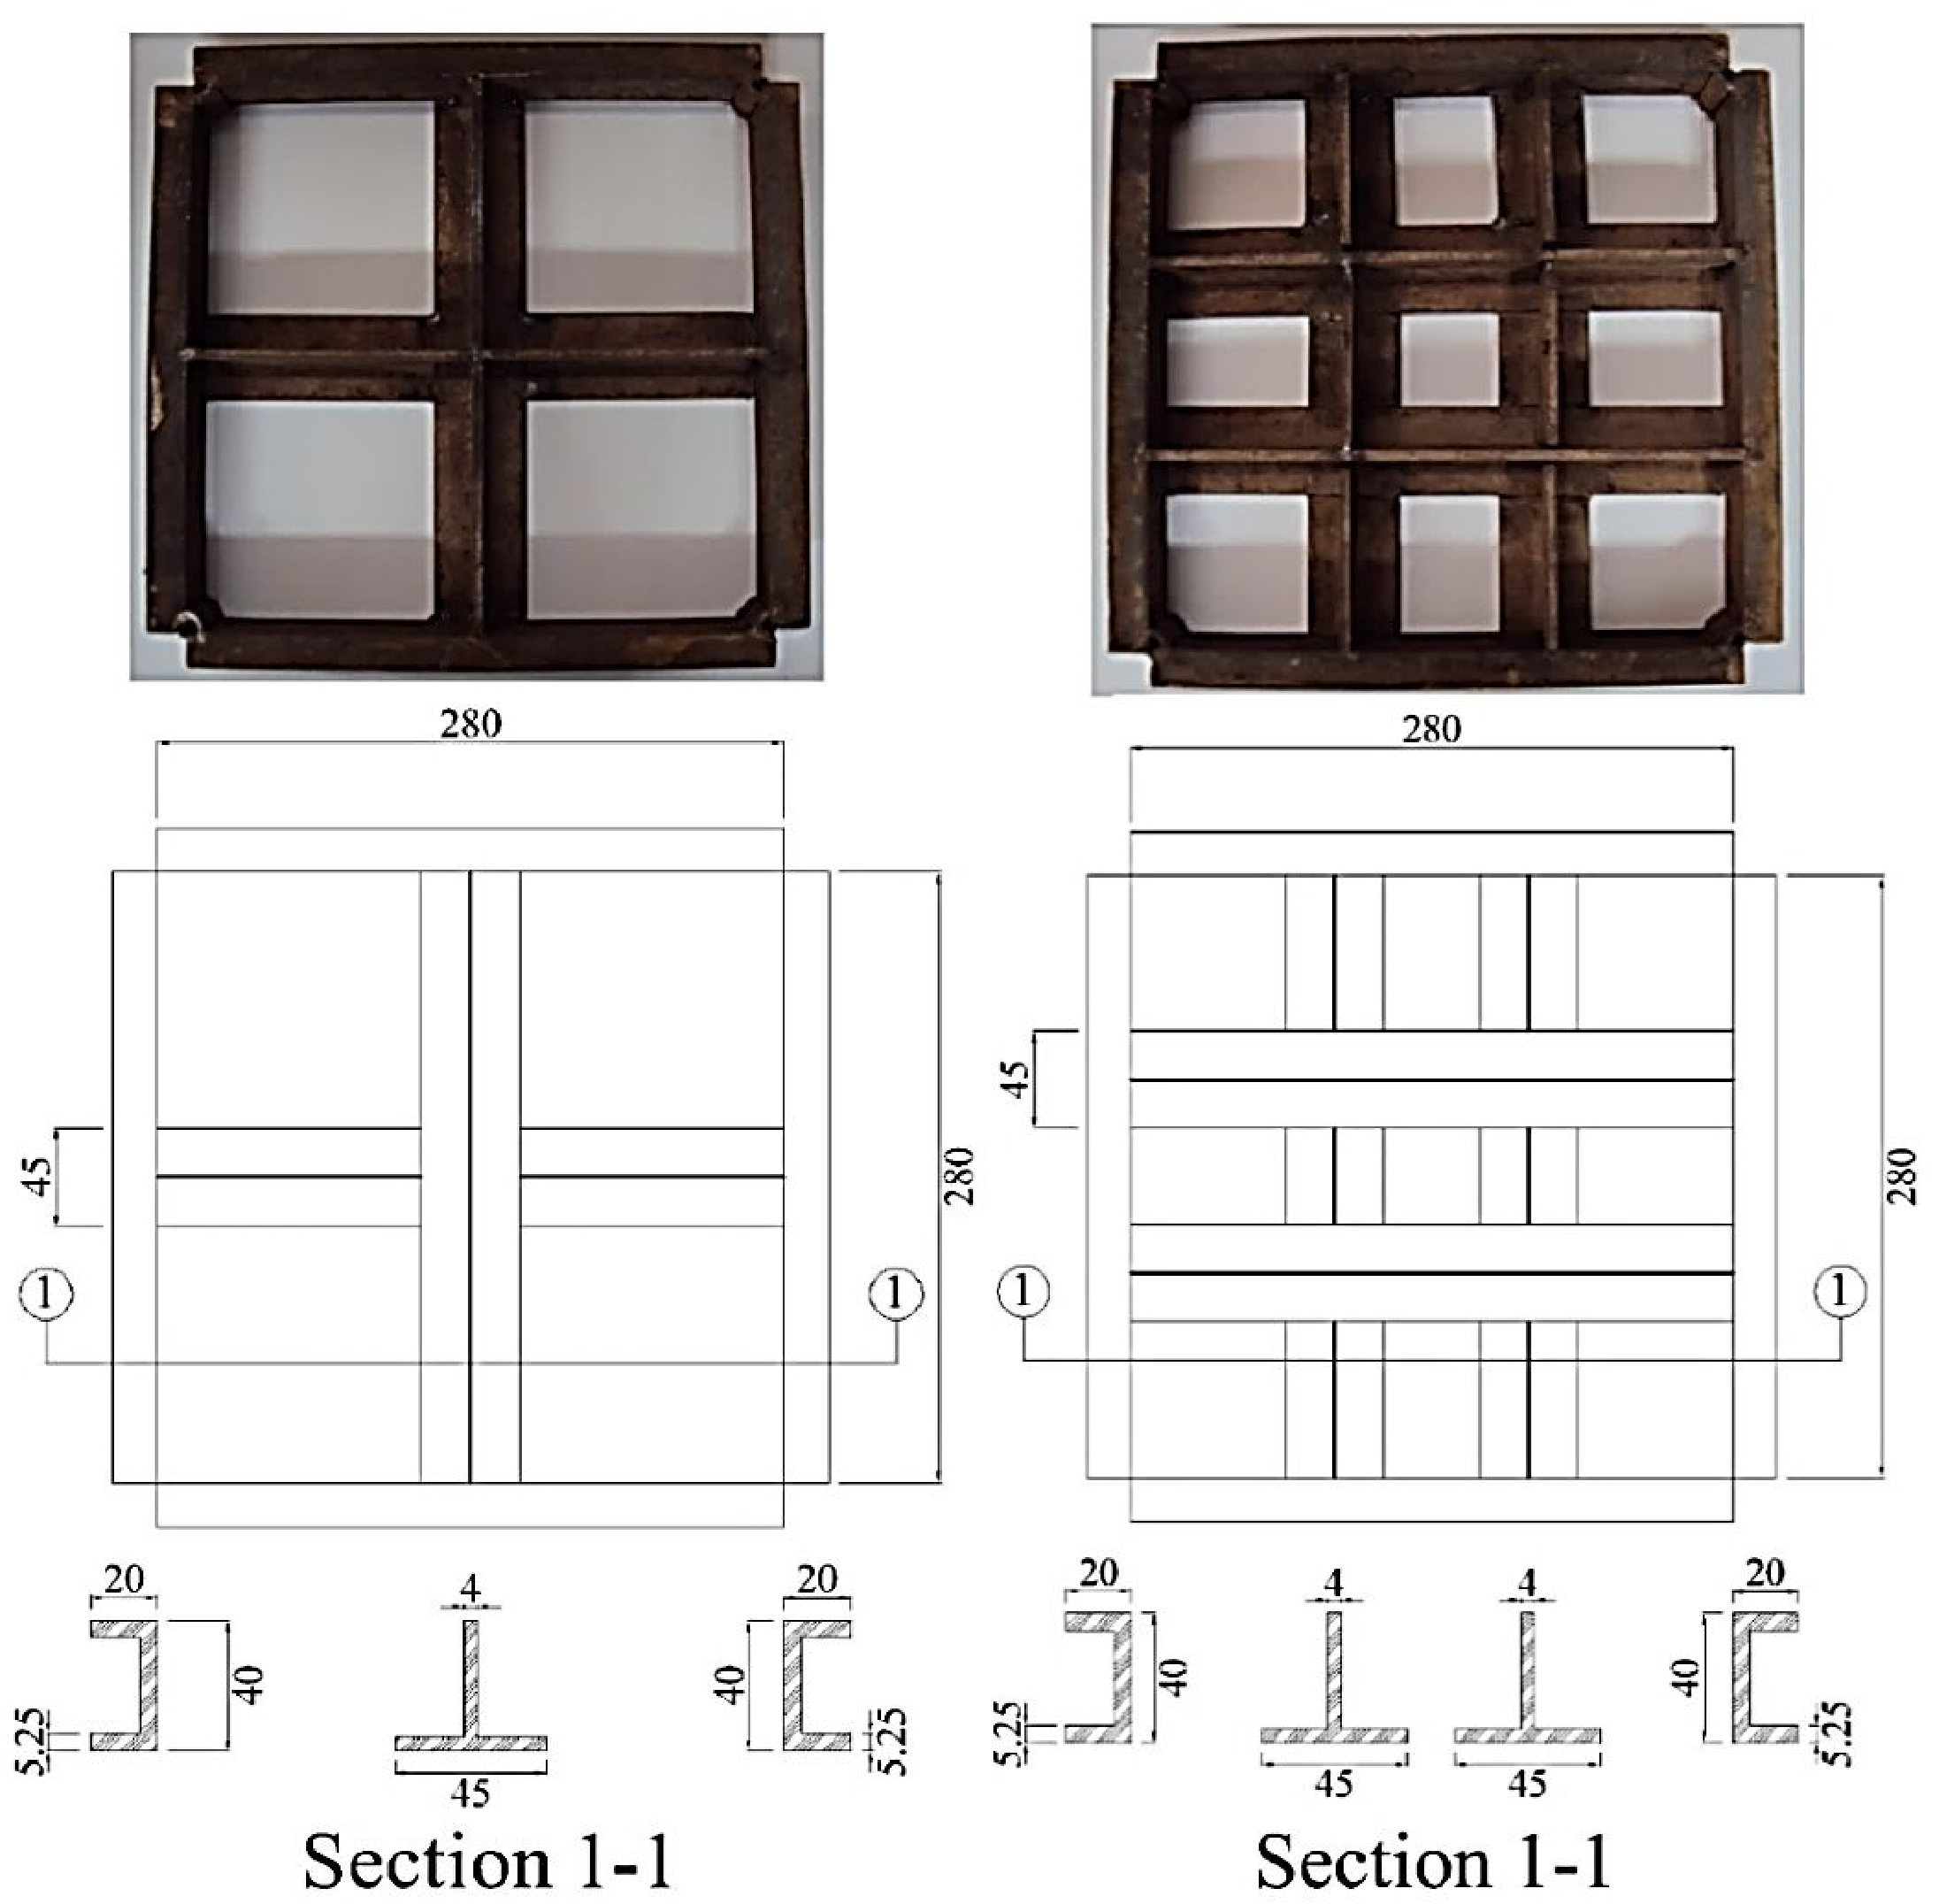
\includegraphics[width=\columnwidth]{ahf5.pdf}};
%\draw (3,0) node [anchor=north,blue]{\LARGE\textbf{a) G2}};
%\draw (9,0) node [anchor=north,blue]{\LARGE\textbf{b) G3}};
%\end{tikzpicture}

\tikzsetnextfilename{b16if1}
\begin{tikzpicture}
\draw (0,0) node [anchor=south west] {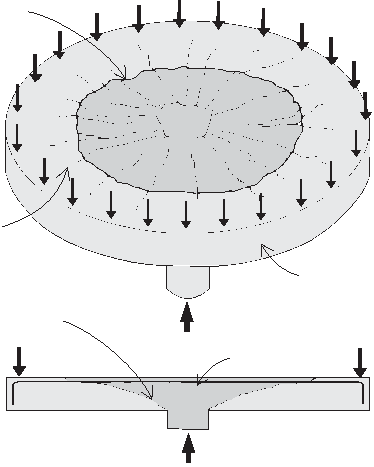
\includegraphics[width=\columnwidth]{b16if1.pdf}};
\draw (3,6) node [blue]{\LARGE\textbf{a)}};
\draw (3,1) node [anchor=north,blue]{\LARGE\textbf{b)}};
\draw (12,4) node [anchor=north west]{\LARGE$\mathbf{q}$};
\draw (0.8,4) node [anchor=north west]{\LARGE$\mathbf{q}$};
\draw (11,14) node [anchor=north west]{\LARGE$\mathbf{q}$};
\draw (6.4,0.5) node [anchor=west]{\LARGE$\mathbf{V}$};
\draw (6.4,4.8) node [anchor=west]{\LARGE$\mathbf{V}$};
\draw (7.4,3.6) node [anchor=west]{\LARGE Punching cone};
\draw (0.7,5) node []{\LARGE Punching};
\draw (0.7,4.5) node []{\LARGE shear crack};
\draw (9.8,6) node [anchor=south west]{\LARGE Flat slab};
\draw (-1,8.3) node []{\LARGE Flexural};
\draw (-1,7.8) node []{\LARGE crack};
\draw (-0.4,15) node []{\LARGE Punching};
\draw (-0.4,14.5) node []{\LARGE shear crack};
%\draw[help lines,red] (0,0) grid (12,15);
\end{tikzpicture}

%\tikzsetnextfilename{b16if2}
%\begin{tikzpicture}
%\draw (0,0) node [anchor=south west] {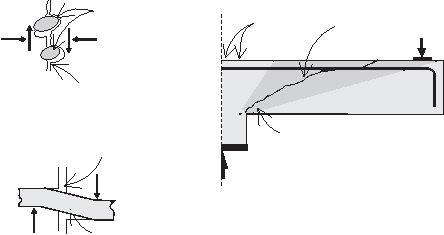
\includegraphics[width=\columnwidth]{b16if2.pdf}};
%\draw (2,3.8) node [anchor=north,blue]{\Large\textbf{a)}};
%\draw (2,0) node [anchor=north,blue]{\Large\textbf{b)}};
%\draw (9,2) node [anchor=north,blue]{\Large\textbf{c)}};
%\draw (9.3,3.3) node [anchor=north]{\Large Compressive};
%\draw (9.3,2.8) node [anchor=north]{\Large stress field};
%\draw (9.3,6.3) node [anchor=west]{\Large Punching};
%\draw (9.3,5.8) node [anchor=west]{\Large shear crack};
%\draw (6.2,1.5) node [anchor=west]{\LARGE $\mathbf{V}$};
%\draw (7,6.3) node [anchor=west]{\Large Flexural};
%\draw (7,5.8) node [anchor=west]{\Large cracks};
%\draw (2.5,6) node [anchor=south west]{\Large Aggregates};
%\draw (2.4,5.6) node [anchor=west]{\LARGE $\sigma_\mathrm{agg}$};
%\draw (2,5) node [anchor=west]{\LARGE $\tau_\mathrm{agg}$};
%\draw (0.3,5.1) node []{\LARGE $\sigma_\mathrm{agg}$};
%\draw (0.4,6) node []{\LARGE $\tau_\mathrm{agg}$};
%\draw (2,4) node []{\Large Crack interface};
%\draw (3,2.2) node [anchor = south]{\Large Crack interface};
%\draw (2.8,1) node [anchor=south west]{\LARGE $\mathbf{V}_\mathrm{dow}$};
%\draw (1.1,0) node [anchor=south east]{\LARGE $\mathbf{V}_\mathrm{dow}$};
%\draw (2.6,0) node [anchor = west]{\Large Dowel bar};
%\draw (6.2,6) node []{\Large C};
%\draw (6.25,5.9) node []{\Large L};
%%\draw[help lines,red] (0,0) grid (12,8);
%\end{tikzpicture}

%\tikzsetnextfilename{b16if3}
%\begin{tikzpicture}
%\draw (0,0) node [anchor=south west] {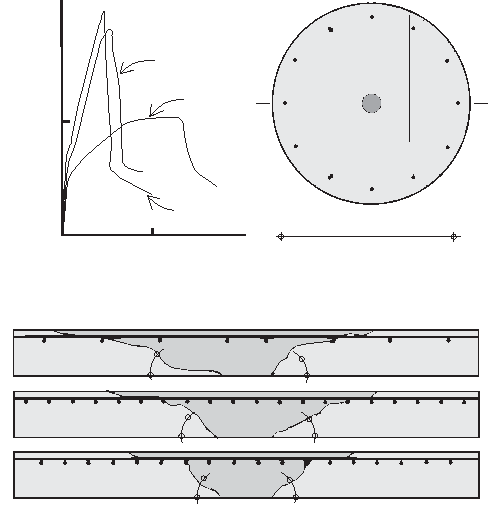
\includegraphics[width=\columnwidth]{b16if3.pdf}};
%\draw (4,6) node [anchor=north,blue]{\Large\textbf{a)}};
%\draw (9.5,6) node [anchor=north,blue]{\Large\textbf{b)}};
%\draw (6,0) node [anchor=south,blue]{\Large\textbf{c)}};
%\draw (.5,5) node [anchor=south west]{\Large a-a};
%\draw (.5,3.9) node [anchor=south west]{\large HSC9-24$^\circ$};
%\draw (.5,2.3) node [anchor=south west]{\large HSC0-29$^\circ$};
%\draw (.5,0.9) node [anchor=south west]{\large HSC4-45$^\circ$};
%
%\draw (3.8,3.75) node [anchor=south west,rotate=72]{\large 18$^\circ$};
%\draw (8,3.65) node [anchor=south east,rotate=-60]{\large 30$^\circ$};
%\draw (4.5,2.2) node [anchor=south west,rotate=58]{\large 32$^\circ$};
%\draw (8.2,2.1) node [anchor=south east,rotate=-65]{\large 25$^\circ$};
%\draw (4.6,0.75) node [anchor=south west,rotate=45]{\large 45$^\circ$};
%\draw (7.9,0.65) node [anchor=south east,rotate=-45]{\large 45$^\circ$};
%
%\draw (12,0.9) node [anchor=south east]{\large $\rho=1.19\%$};
%\draw (12,2.3) node [anchor=south east]{\large $\rho=0.80\%$};
%\draw (12,3.9) node [anchor=south east]{\large $\rho=0.33\%$};
%
%\draw (11.8,10.7) node [anchor=south west]{\Large a};
%\draw (6.9,10.7) node [anchor=south east]{\Large a};
%\draw (9.5,7.3) node [anchor=south]{\Large 2400mm};
%\draw (6.3,7.4) node [anchor=north east]{\large 0.02};
%\draw (4,7.4) node [anchor=north ]{\large 0.01};
%\draw (4,6.7) node [anchor=north ]{\Large $\delta/l_\mathrm{s}$};
%\draw (0.5,10.2) node [rotate=90]{\Large $\mathbf{V/(I_0d\sqrt[3]{f_c})},\sqrt[3]{\mathrm{MPa}}$};
%\draw (5,8) node [ ]{\large HSC4};
%\draw (5.3,10.8) node [ ]{\large HSC9};
%\draw (4.6,11.8) node [ ]{\large HSC0};
%
%\draw (1.2,13) node []{\large 0.40};
%\draw (1.2,10.2) node []{\large 0.20};
%\draw (1.3,7.4) node []{\large 0};
%\draw (1.35,7.4) node [anchor = north west]{\large 0};
%
%%\draw[help lines,red] (0,0) grid (12,12);
%\end{tikzpicture}

%\tikzsetnextfilename{c2020f2}
%\begin{tikzpicture}
%\draw (0,0) node [anchor=south west] {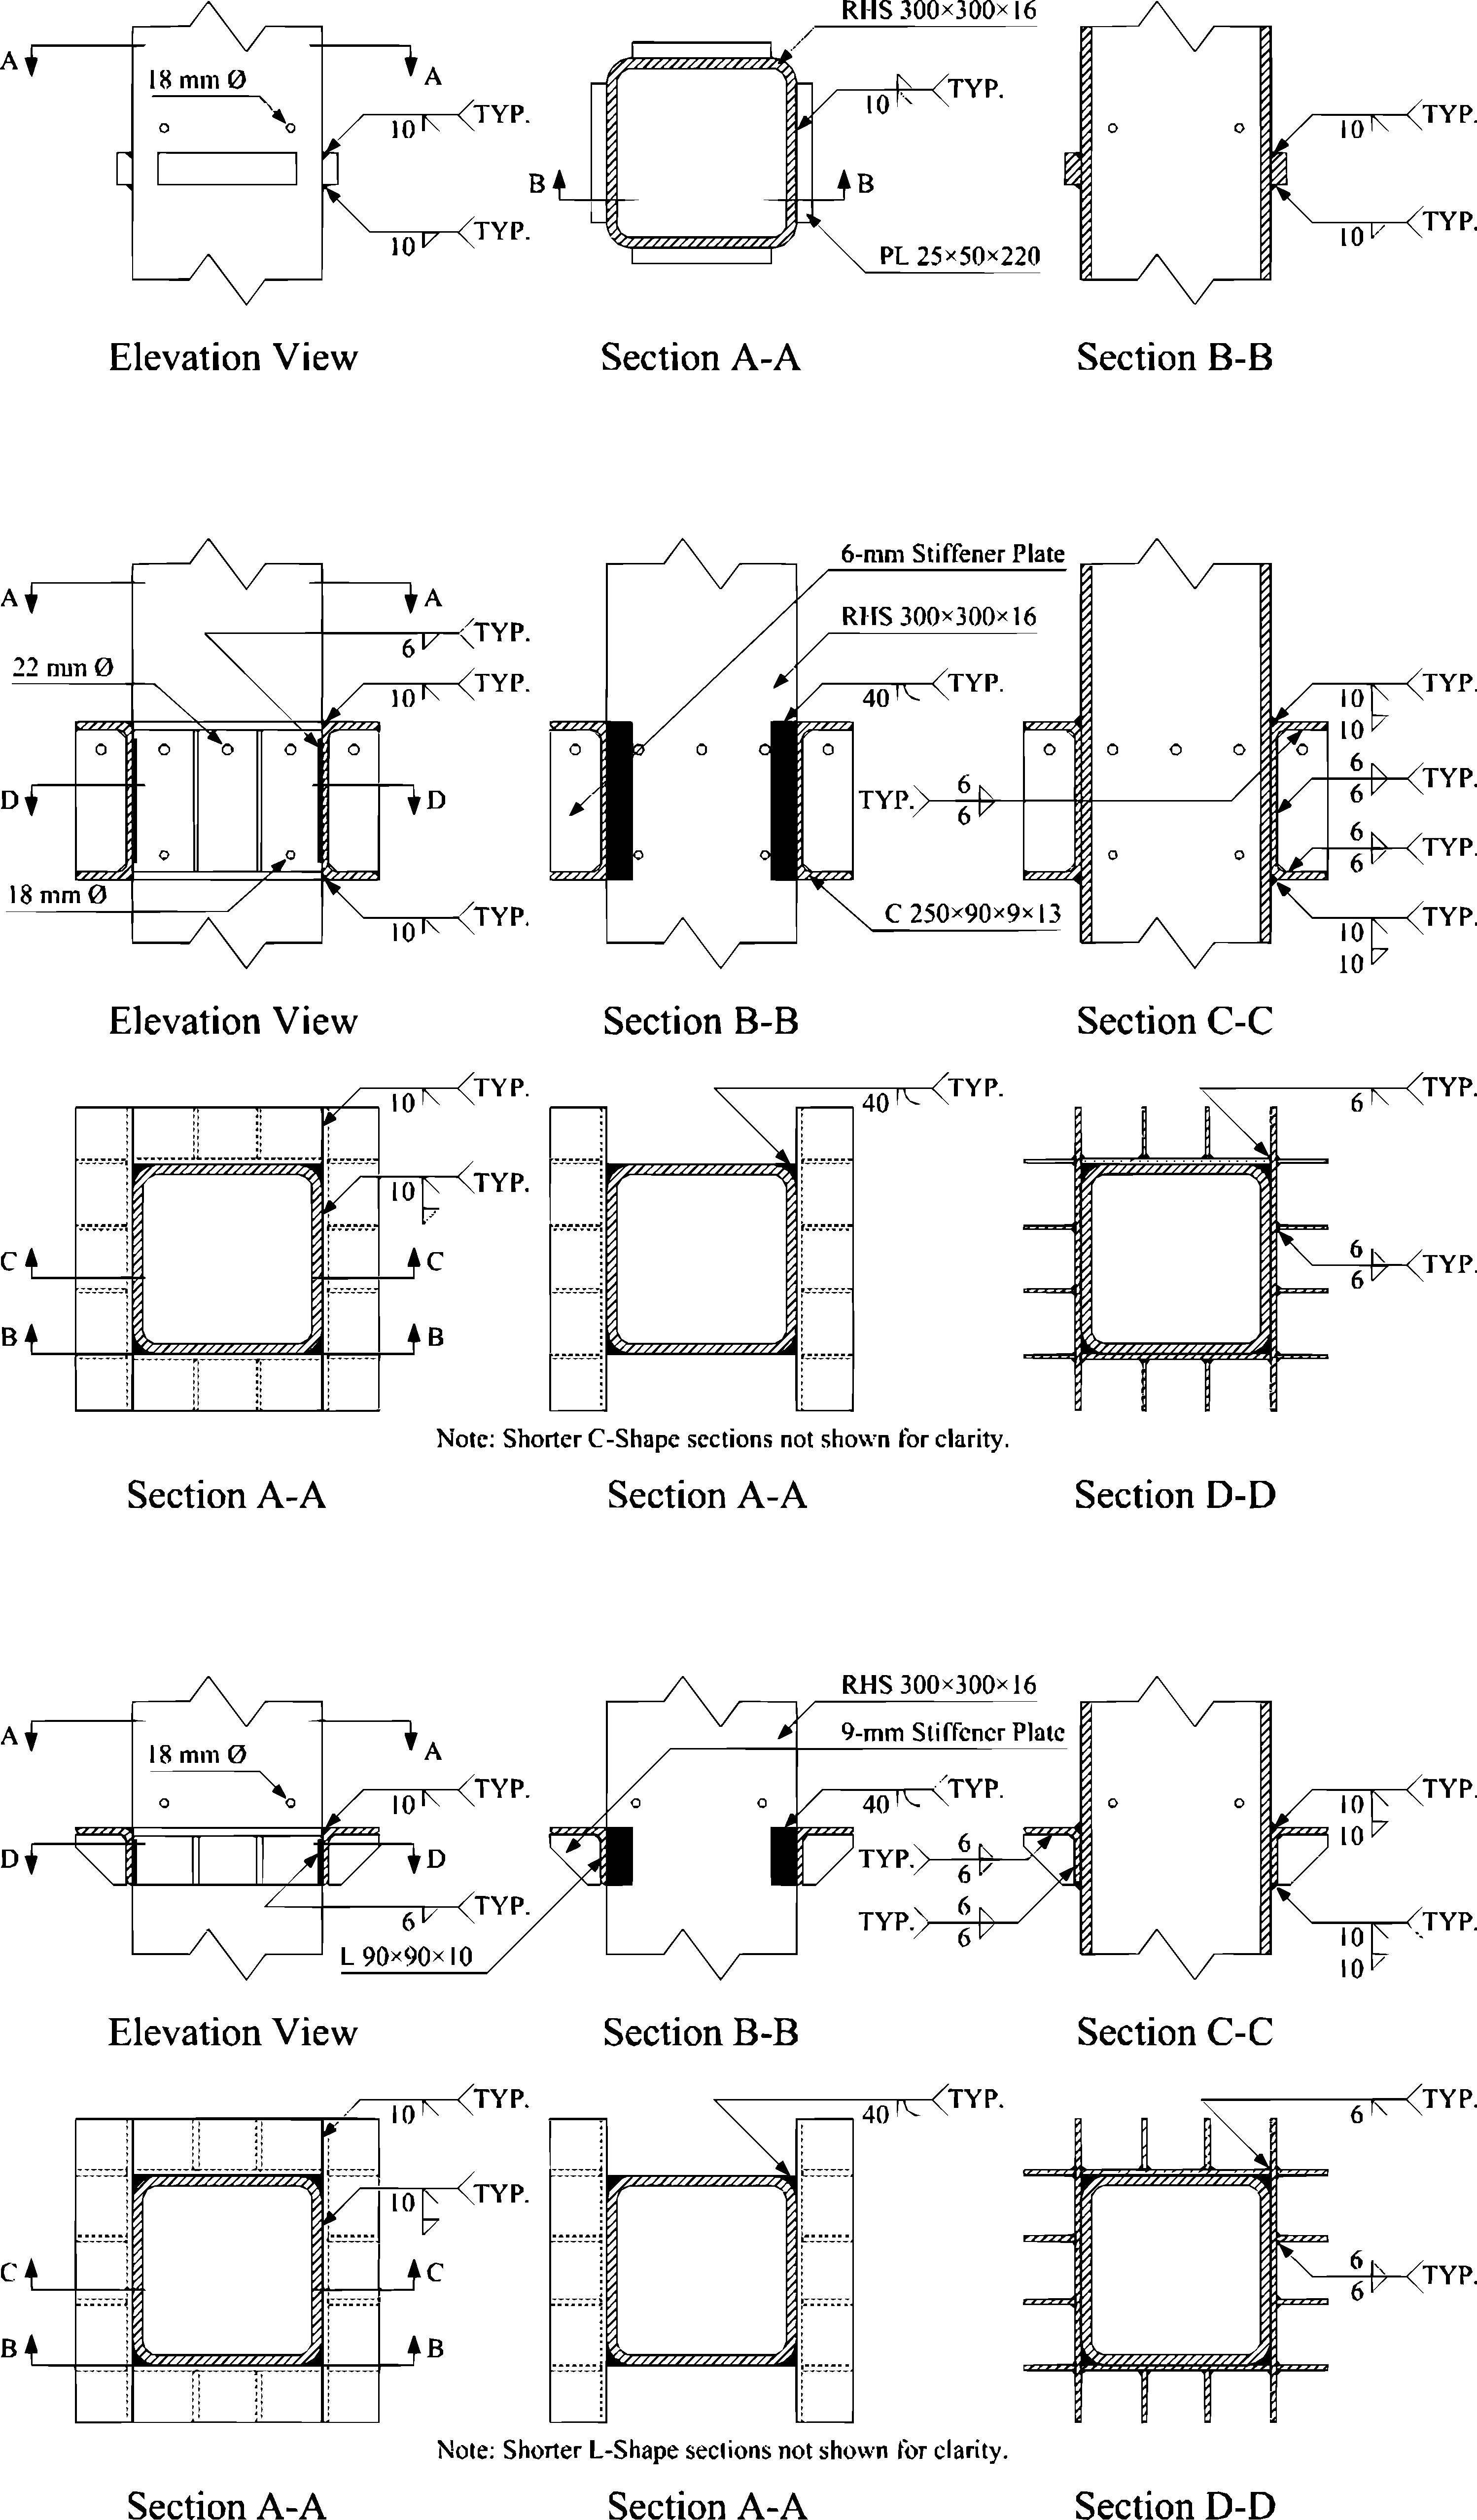
\includegraphics[width=\columnwidth]{c2020f2.pdf}};
%\draw (6,17) node [blue]{\Large\textbf{a) CFT300\_P}};
%\draw (6,8) node [anchor=north,blue]{\Large\textbf{b) CFT300\_C}};
%\draw (6,0) node [anchor=north,blue]{\Large\textbf{c) CFT300\_A}};
%%\draw[help lines,red] (0,0) grid (12,18);
%\end{tikzpicture}

%\tikzsetnextfilename{c2020f3}
%\begin{tikzpicture}
%\draw (0,0) node [anchor=south west] {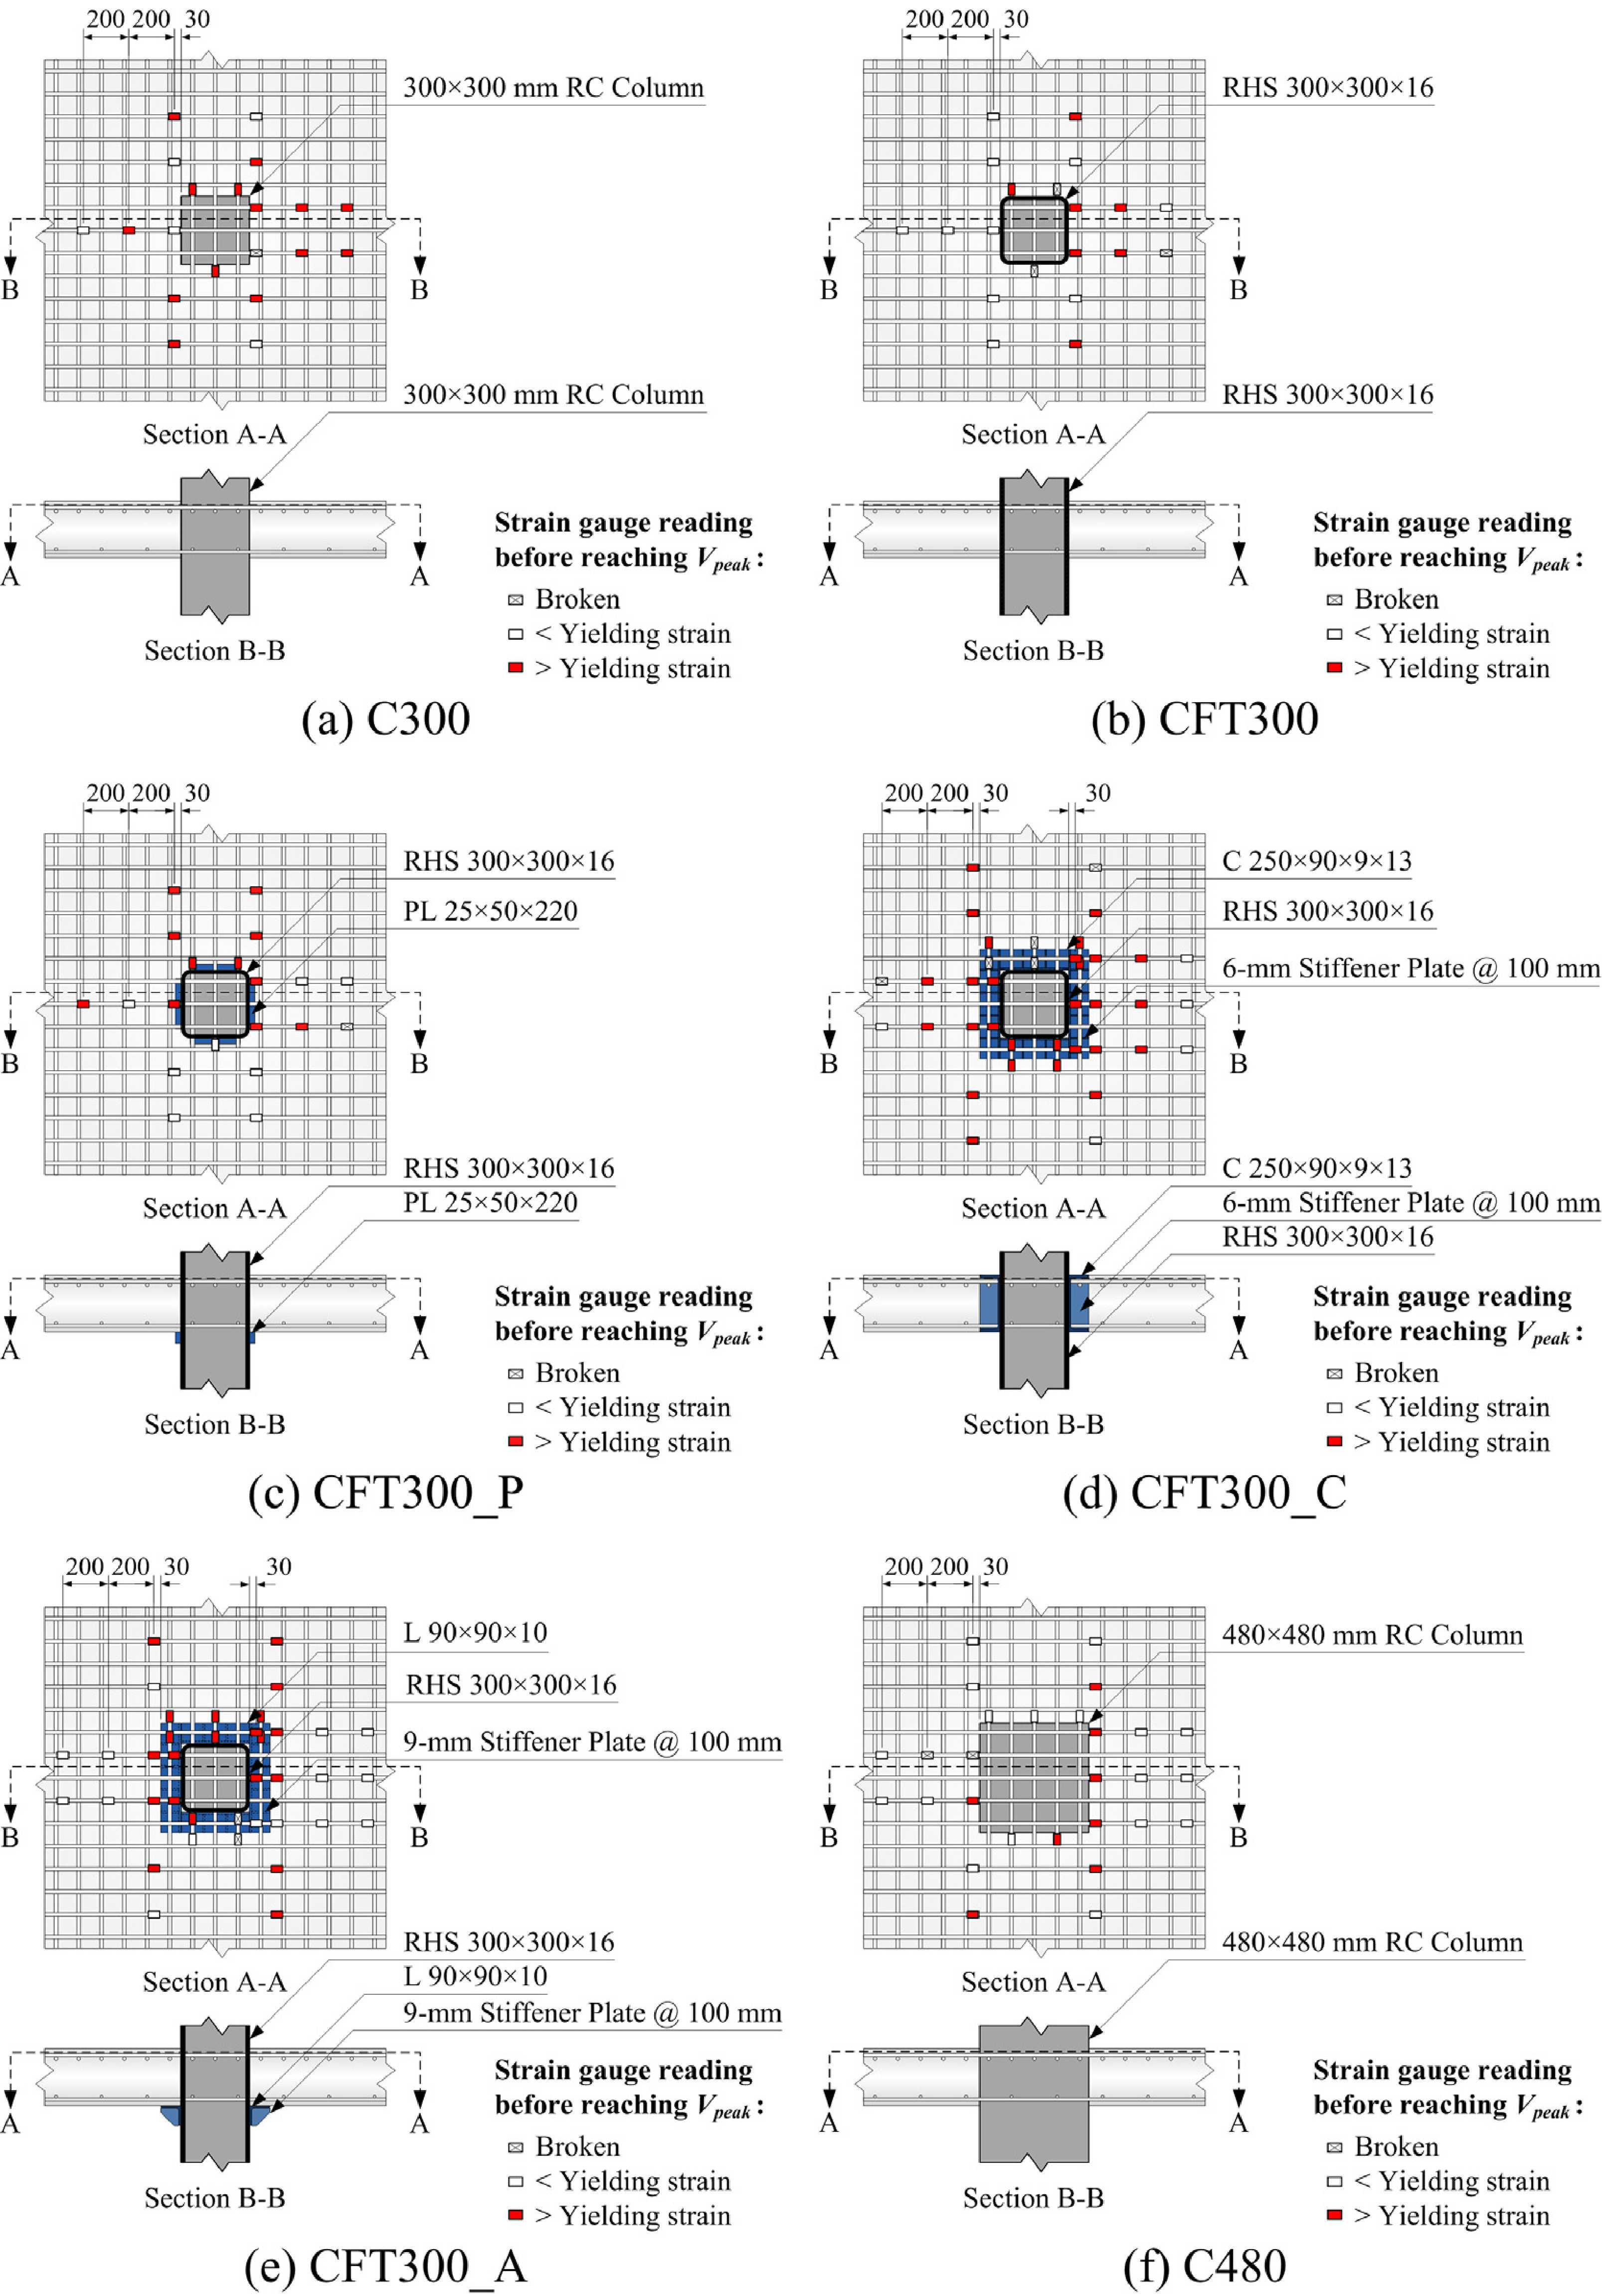
\includegraphics[width=\columnwidth]{c2020f3.pdf}};
%\draw (3,11.95) node [fill=white,white]{\textbf{a) C300}};
%\draw (3,11.95) node [blue]{\textbf{a) C300}};
%\draw (9.2,11.95) node [fill = white,white]{\textbf{b) CFT300}};
%\draw (9.2,11.95) node [blue]{\textbf{b) CFT300}};
%\draw (3,5.95) node [anchor=south,fill=white,white]{\textbf{c) CFT300\_P}};
%\draw (3,5.95) node [anchor=south,blue]{\textbf{c) CFT300\_P}};
%
%\draw (9.2,5.95) node [anchor=south,fill=white,white]{\textbf{d) CFT300\_C}};
%\draw (9.2,5.95) node [anchor=south,blue]{\textbf{d) CFT300\_C}};
%
%\draw (3,-0.05) node [anchor=south,fill=white,white]{\textbf{e) CFT300\_A}};
%\draw (3,-0.05) node [anchor=south,blue]{\textbf{e) CFT300\_A}};
%
%\draw (9.2,-0.05) node [anchor=south,fill=white,white]{\textbf{f) C480}};
%\draw (9.2,-0.05) node [anchor=south,blue]{\textbf{f) C480}};
%
%%\draw[help lines,red] (0,0) grid (12,18);
%\end{tikzpicture}
\end{document}